\chapter{Defining colorings}

\section{The general concept of coloring}

As we will be working with many different colorings, to avoid repetition, we will define the notion of an abstract coloring which all the particular colorings will share.

\begin{definition}
    A \textit{partial function} is a function $f:X \rightarrow Y$ s.t. $\forall x \in X$ we have $f(x) \in Y$ or $f(x)$ is undefined.
\end{definition}

Since we will be working with graphs of Platonic and Archimedean solids, which are all planar. We can define the coloring directly on their plane graphs, as they are drawn on the plane, instead of considering their abstract graphs.

\begin{definition}
    Let $S$ be a set and $G=(V,E,F)$ a plane graph. We define \textit{coloring} of $G$ as a partial function $c: V \cup E \cup F \rightarrow S$ with a coloring rule $R$ that restricts, which elements of the graph cannot be mapped to same element in S.
\end{definition}

In other words, coloring is an assignment of elements in $S$ to vertices, edges or faces of some plane graph. We can think of elements of $S$ as colors but usually, we will use numbers instead. What is especially important to us is, whether any two elements are mapped onto a same target i.e. colored by the same color. The coloring rule then prevents some assignments to be considered valid. This makes the coloring problem non-trivial.

\begin{definition}
    Let the set of all colorings sharing the same coloring rule $R$ be called a \textit{family of colorings}.
\end{definition}

\begin{definition}
    Let $G=(V,E,F)$ a plane graph. Let $C$ be a family of colorings. Let $S$ be a set s.t. $|S| = k$ for some $k \in \mathbb{N}$. A function $c \in C$ such that $c: V \cup E \cup F \rightarrow S$ is called a \textit{k-coloring} of $G$.
\end{definition}

Note that a $k$-coloring does not necessarily have to use all of the $k$ available colors. Mathematically speaking, a $k$-coloring is not necesserily a surjective function.

\begin{definition}
    For a plane graph $G$, family of colorings $C$ and a natural number $k$, if there exists a k-coloring of $G$ then we say that $G$ is \textit{k-colorable}.
\end{definition}

A typical question we ask ourselves when considering colorings of graph is: What is the least amount of colors we can use to color the graph, without breaking the coloring rule? This leads to a definition of so called \textit{chromatic number}. 


\begin{definition}
    For a plane graph $G$ and a family of colorings $C$, let \textit{chromatic number} $\chi ^C (G)$ be the minimum $k \in \mathbb{N}$ s.t. $G$ is k-colorable.
\end{definition}

%\todo[inline]{JH: Přidána poslední věta}
Once we know a graph is k-colorable, there is another interesting property of the graph we can examine. We can ask about how many different colorings with k colors there exists for the given graph. A closely related concept to this question is the \textit{chromatic polynomial}. But first, we need to define what it means for to colorings to be different.

\begin{definition}
    Given a plane graph $G=(V,E,F)$, family of colorings $C$ and k-colorings $c_1,c_2 \in C$: $c_1$ and $c_2$ are different if there exists $x \in V \cup E \cup F$ s.t. $c_1(x) \neq c_2(x)$.
\end{definition}

The definition above states, that if two colorings assign some element a different color, then the colorings are considered different. Note that this does not take into account any symmetries of the graph.

\begin{definition}
    For graph $G$ and a family of colorings $C$, the \textit{chromatic polynomial} denoted by $P_{C}(G,x)$ is a function s.t. $\forall k \in \mathbb{N} : P_C(G,k) = n$, where $n$ is the number of different k-colorings of $G$.
\end{definition}

\section{Particular types of colorings}

\subsection{Vertex coloring}

\begin{definition}
    Given set $S$ a \textit{vertex coloring} of a plane graph $G=(V,E,F)$ is any coloring $c : V \rightarrow S$ belonging to family of colorings with the following coloring rule:
    \begin{equation}\label{eqn:vtx_rule}
        \forall u,v \in V, \quad \text{if } \{u,v\} \in E, \text{ then } c(u) \neq c(v). 
        \tag{$R_V$}
    \end{equation}
    We will denote this family of colorings by $X$.
\end{definition}

In other words, vertex coloring is an assignment of colors to each vertex s.t. no two vertices connected by an edge share the same color.

\begin{figure}[H]
    \centering
    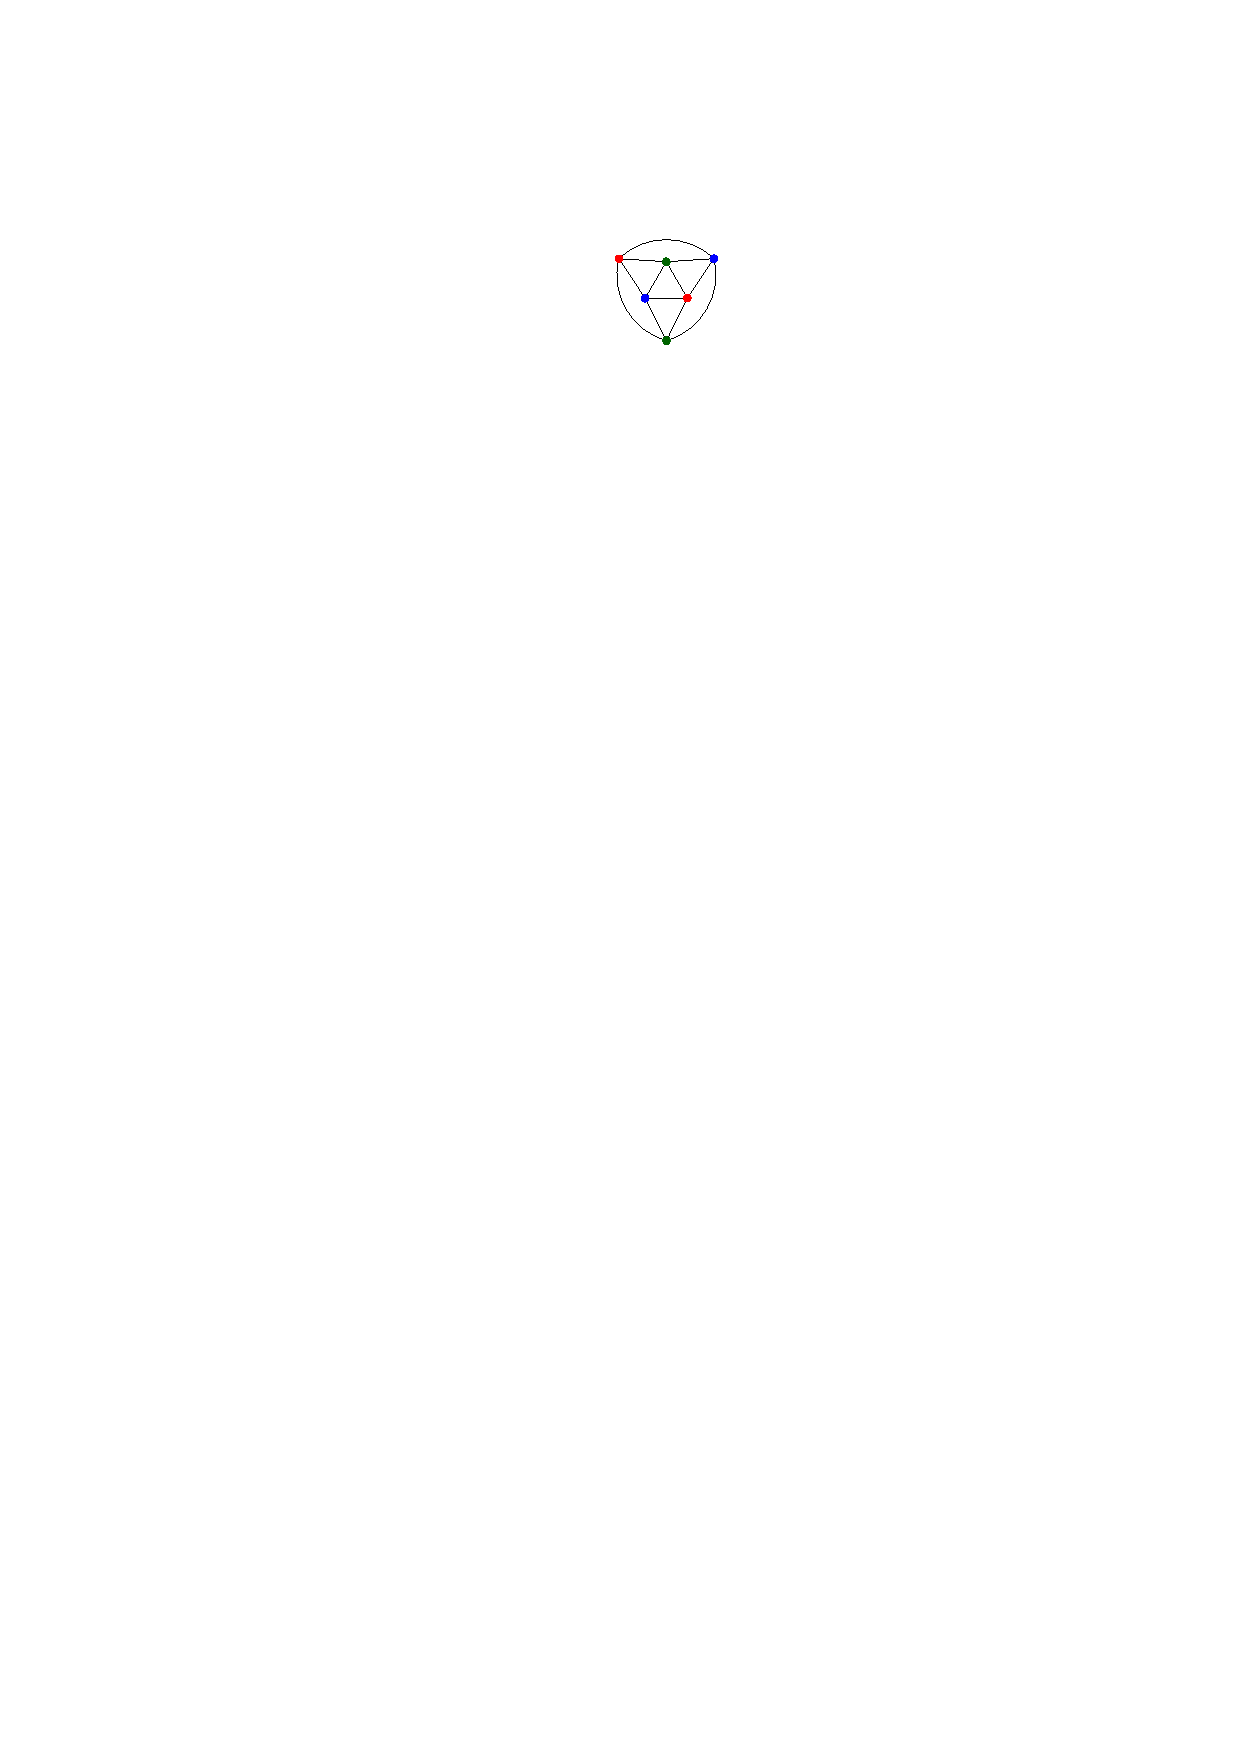
\includegraphics[width=0.2\textwidth]{../Resources/Figs/octahedral_vtx_colr.pdf}
    \caption{Vertex coloring of octahedral graph}
    \label{fig:octahedral_vtx_coloring}
\end{figure}

The graph in figure~\ref{fig:octahedral_vtx_coloring} has vertex chromatic number 3.

\subsection{Edge coloring}

\begin{definition}
    Let $S$ be a set. An \textit{edge coloring} of a plane graph $G=(V,E,F)$ is a coloring $c: E \rightarrow S$ belonging to family of colorings for which the coloring rule is: 
    \begin{equation}\label{eqn:edge_rule}
     \forall e,f \in E, \quad \text{ whenever } e \cap f \neq \emptyset \text{ then } c(e) \neq c(f) \tag{$R_E$}
    \end{equation}
    We will denote this family of colorings by $X'$.
   
\end{definition}

What the definition above says is, that whenever two edges share an endpoint, they cannot share the same color. 

\begin{figure}[H]
    \centering
    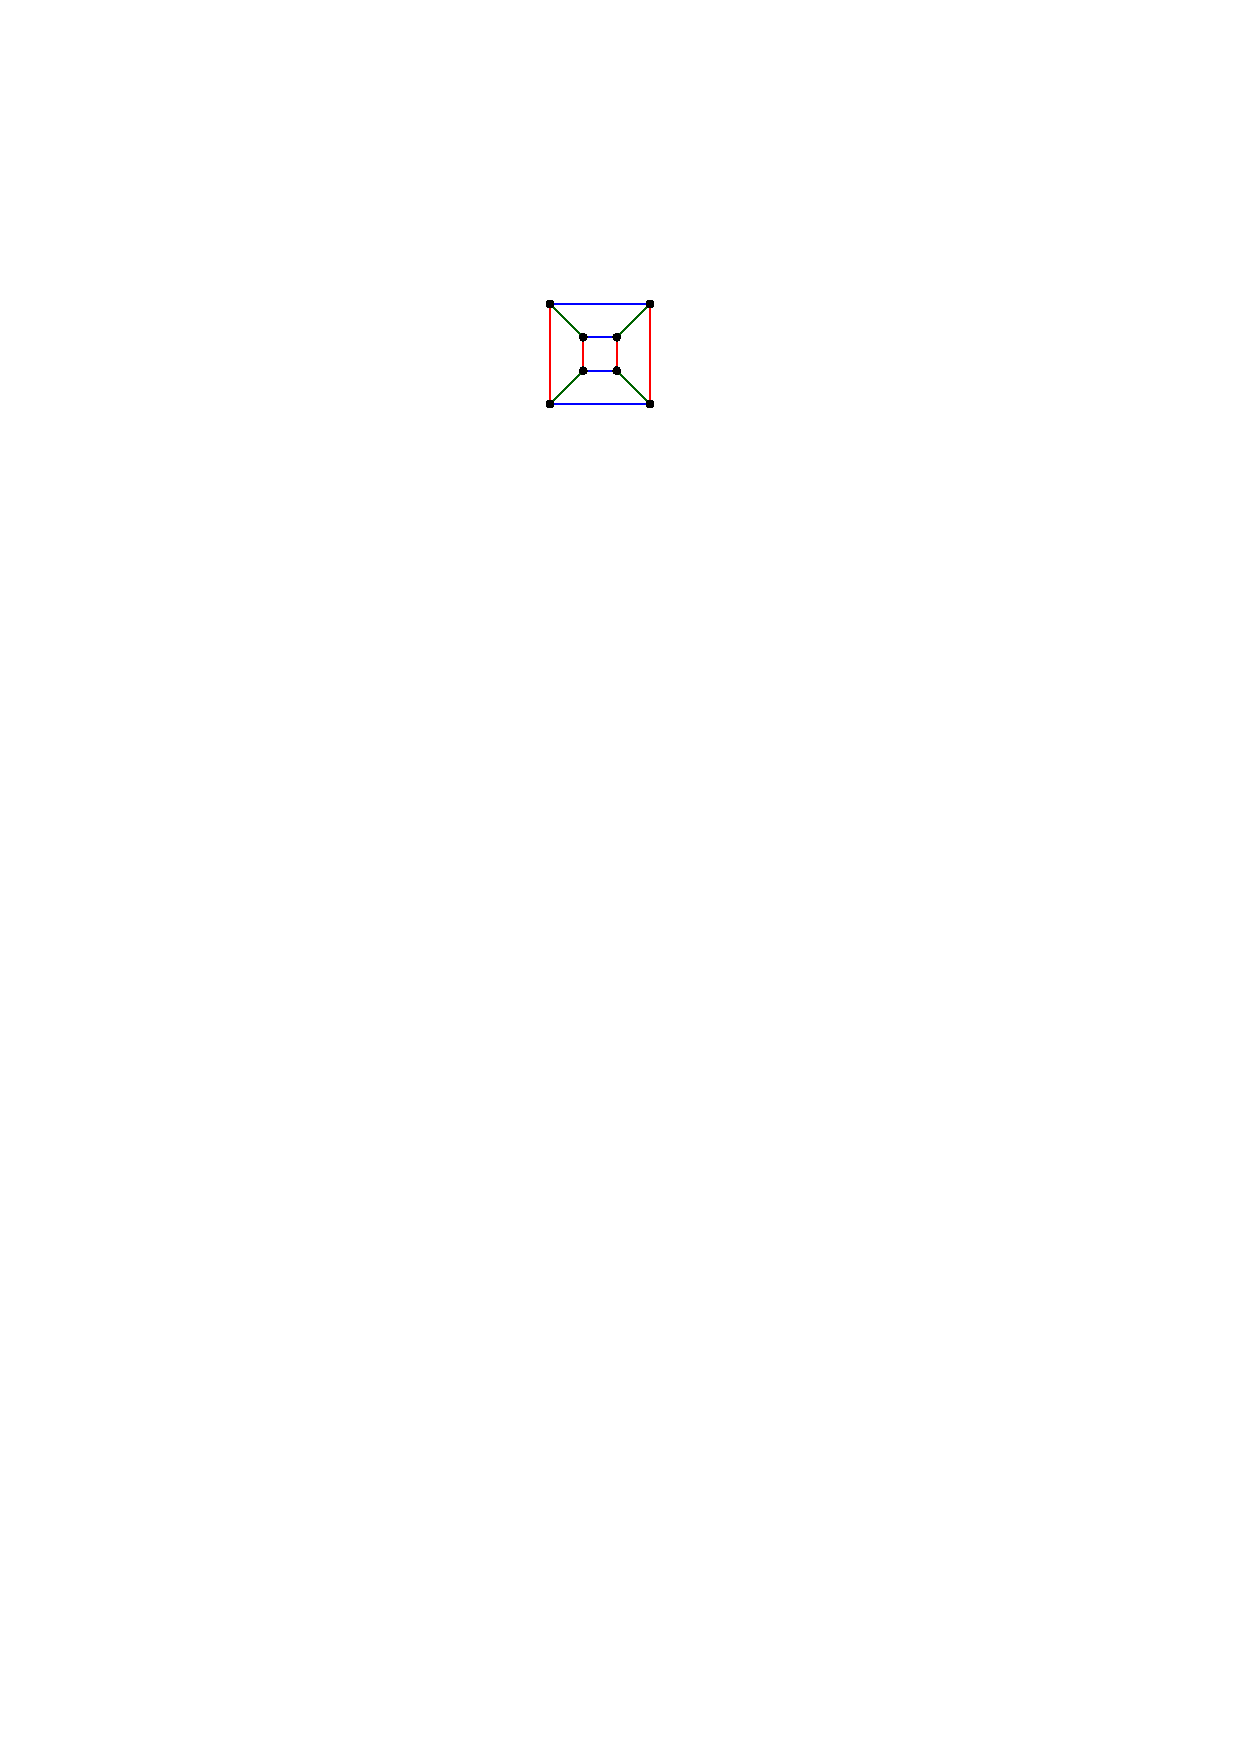
\includegraphics[width=0.2\textwidth]{../Resources/Figs/cubical_edg_colr.pdf}
    \caption{Edge coloring of cubical graph}
    \label{fig:cubical_edge_coloring}
\end{figure}



\subsection{Total coloring}

By combining the colorings above and extending by another restriction, we get a so called \textit{total coloring} \cite{behzad65}.

\begin{definition}
    For some set $S$ a \textit{total coloring} of a plane graph $G=(V,E,F)$ is a coloring $c: V \cup E \rightarrow S$ from family of colorings sharing both coloring rules \ref{eqn:vtx_rule} and \ref{eqn:edge_rule} and the following additional rule: 
    \begin{equation}\label{eqn:tot_rule}
    \forall v \in V,  \forall e \in E, \text{ if } v \in e \text{ then } c(v) \neq c(e) \tag{$R_T$}
    \end{equation}
    We will call this family $X''$.
\end{definition}

\begin{figure}[H]
    \centering
    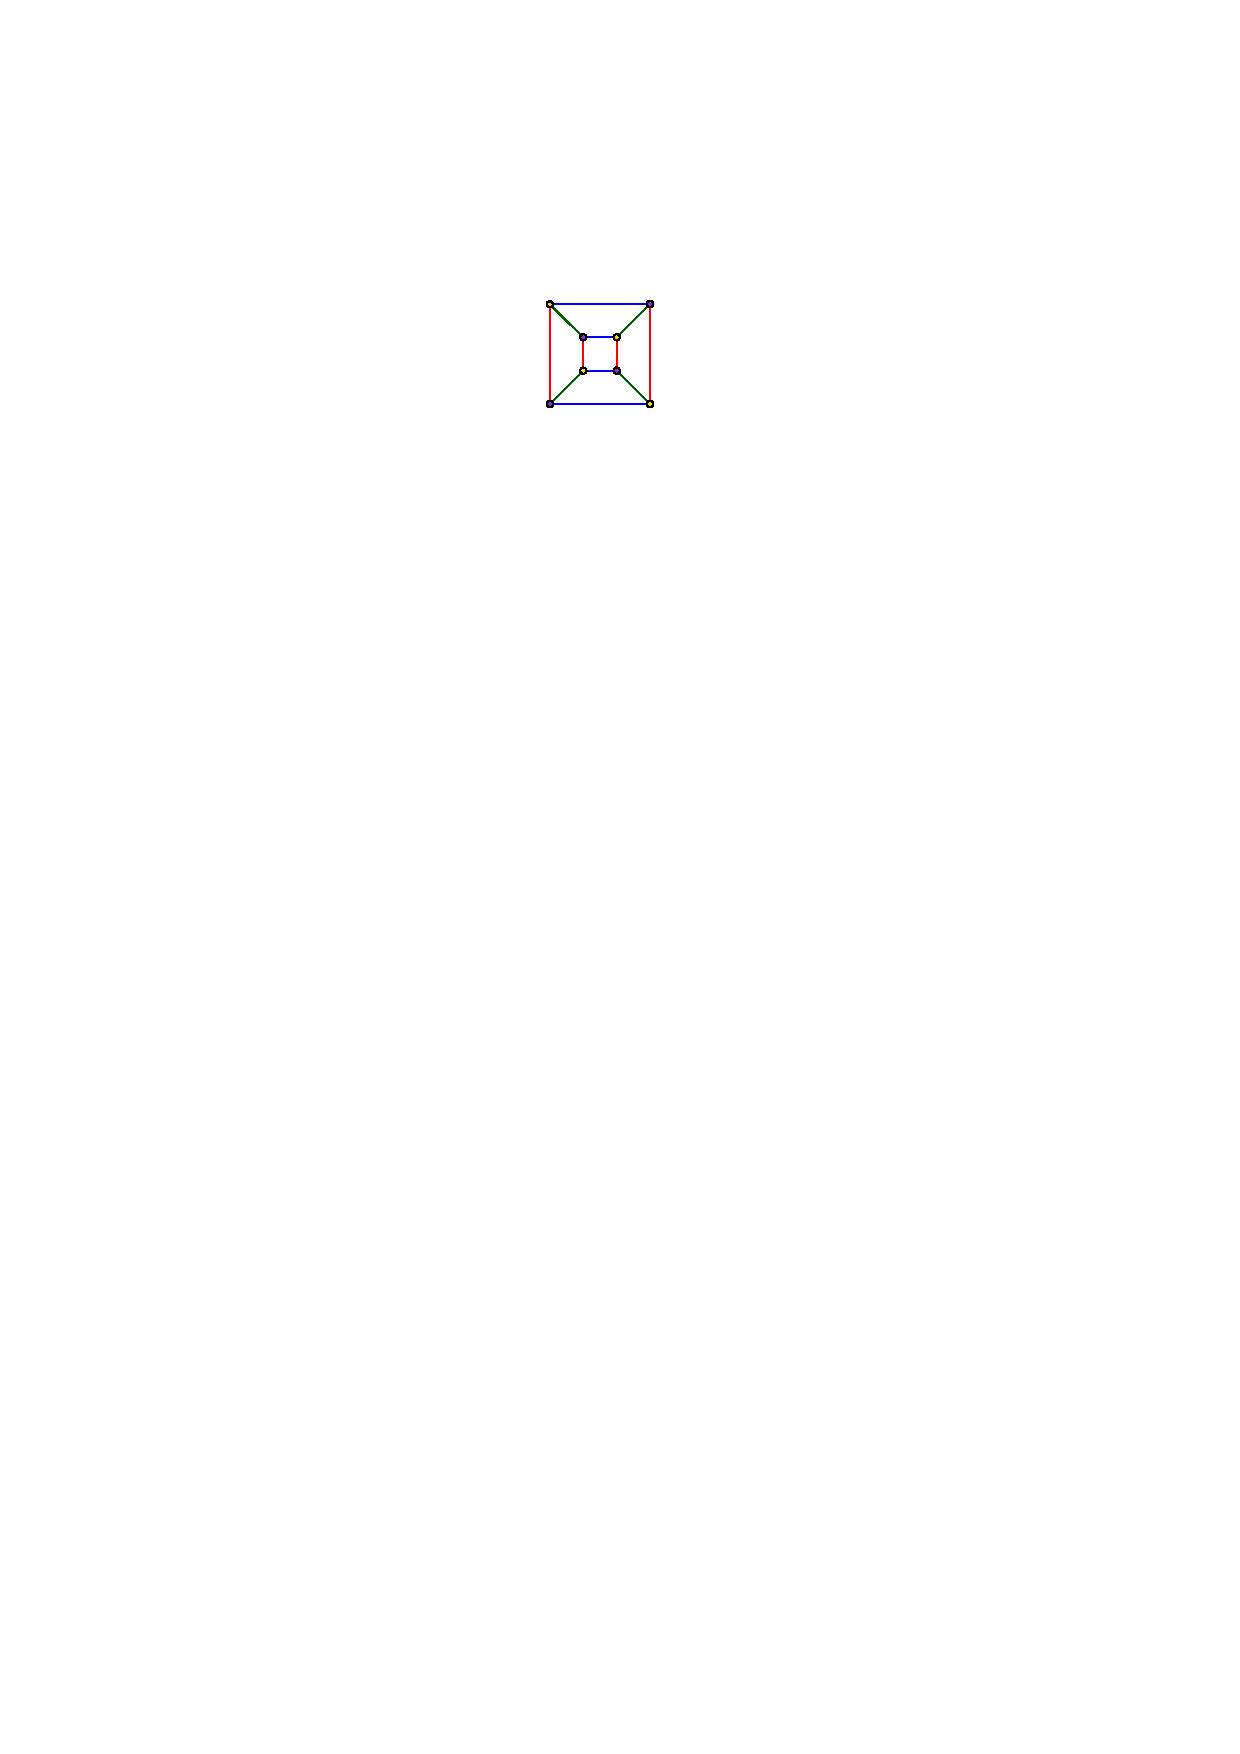
\includegraphics[width=0.2\textwidth]{../Resources/Figs/cubical_tot_colr.pdf}
    \caption{Total coloring of cubical graph using five colors}
    \label{fig:cubical_tot_coloring}
\end{figure}

\begin{figure}[H]
    \centering
    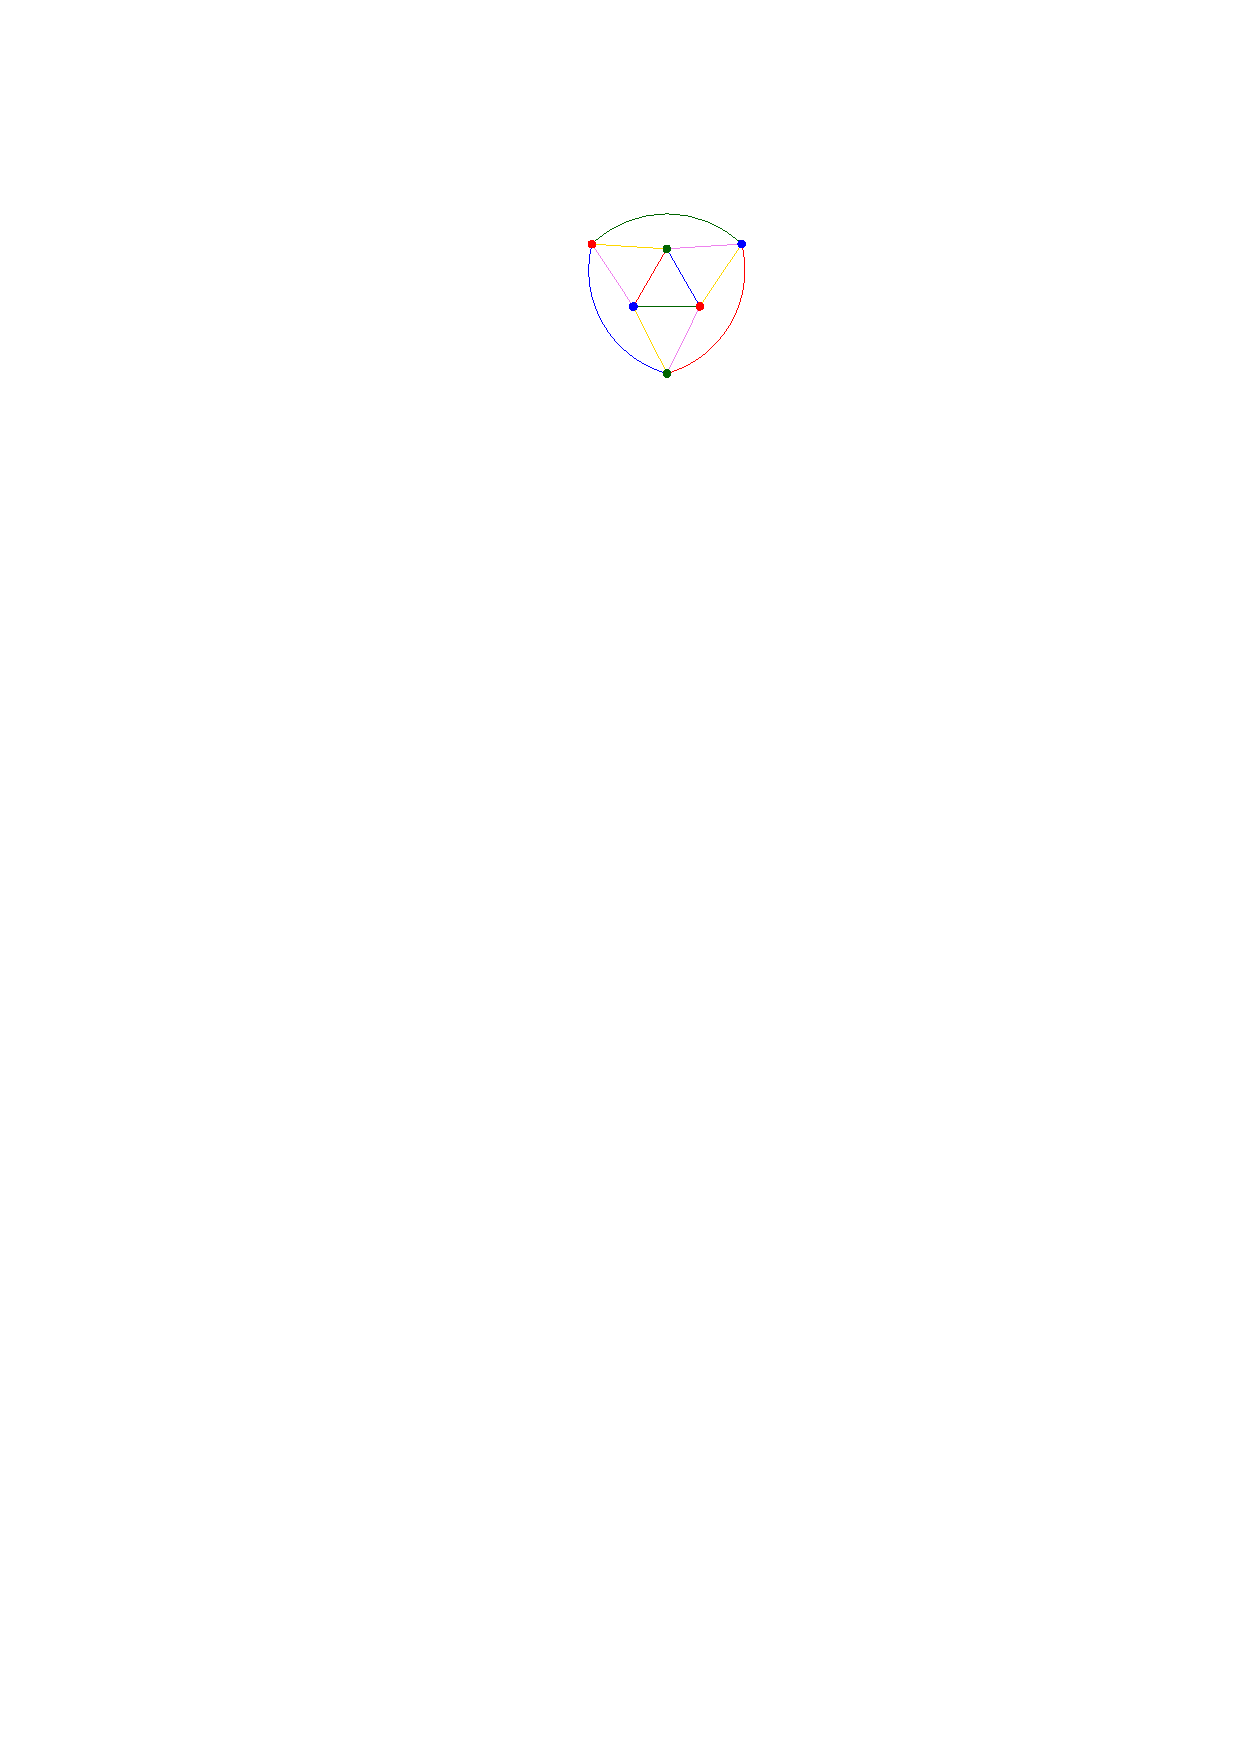
\includegraphics[width=0.2\textwidth]{../Resources/Figs/octahedral_tot_colr.pdf}
    \caption{Total coloring of octahedral graph using five colors}
    \label{fig:octahedral_tot_coloring}
\end{figure}

\subsection{Face coloring}

Since we consider planar graphs, we can also color faces of the corresponding plane graphs.

\begin{definition}
    For a plane graph $G=(V,E,F)$ and a region $R \in F$ we define $\bnd(R)$ as the set of all edges constituting the boundary of $R$.
\end{definition}

\begin{definition}
    For a set $S$ and a plane graph $G=(V,E,F)$ we define \textit{face coloring} as any function $c: F \rightarrow S$ s.t. it belongs to a family of colorings with the following coloring rule:
    \begin{equation}\label{eqn:face_rule}
     \forall R_1,R_2 \in F, \quad \text{ if } \bnd(R_1) \cap \bnd(R_2) \neq \emptyset \text{ then } c(R_1) \neq c(R_2) \tag{$R_F$}
    \end{equation}
    We will denote this family of colorings by $X^F$.
\end{definition}

\begin{figure}[H]
    \centering
    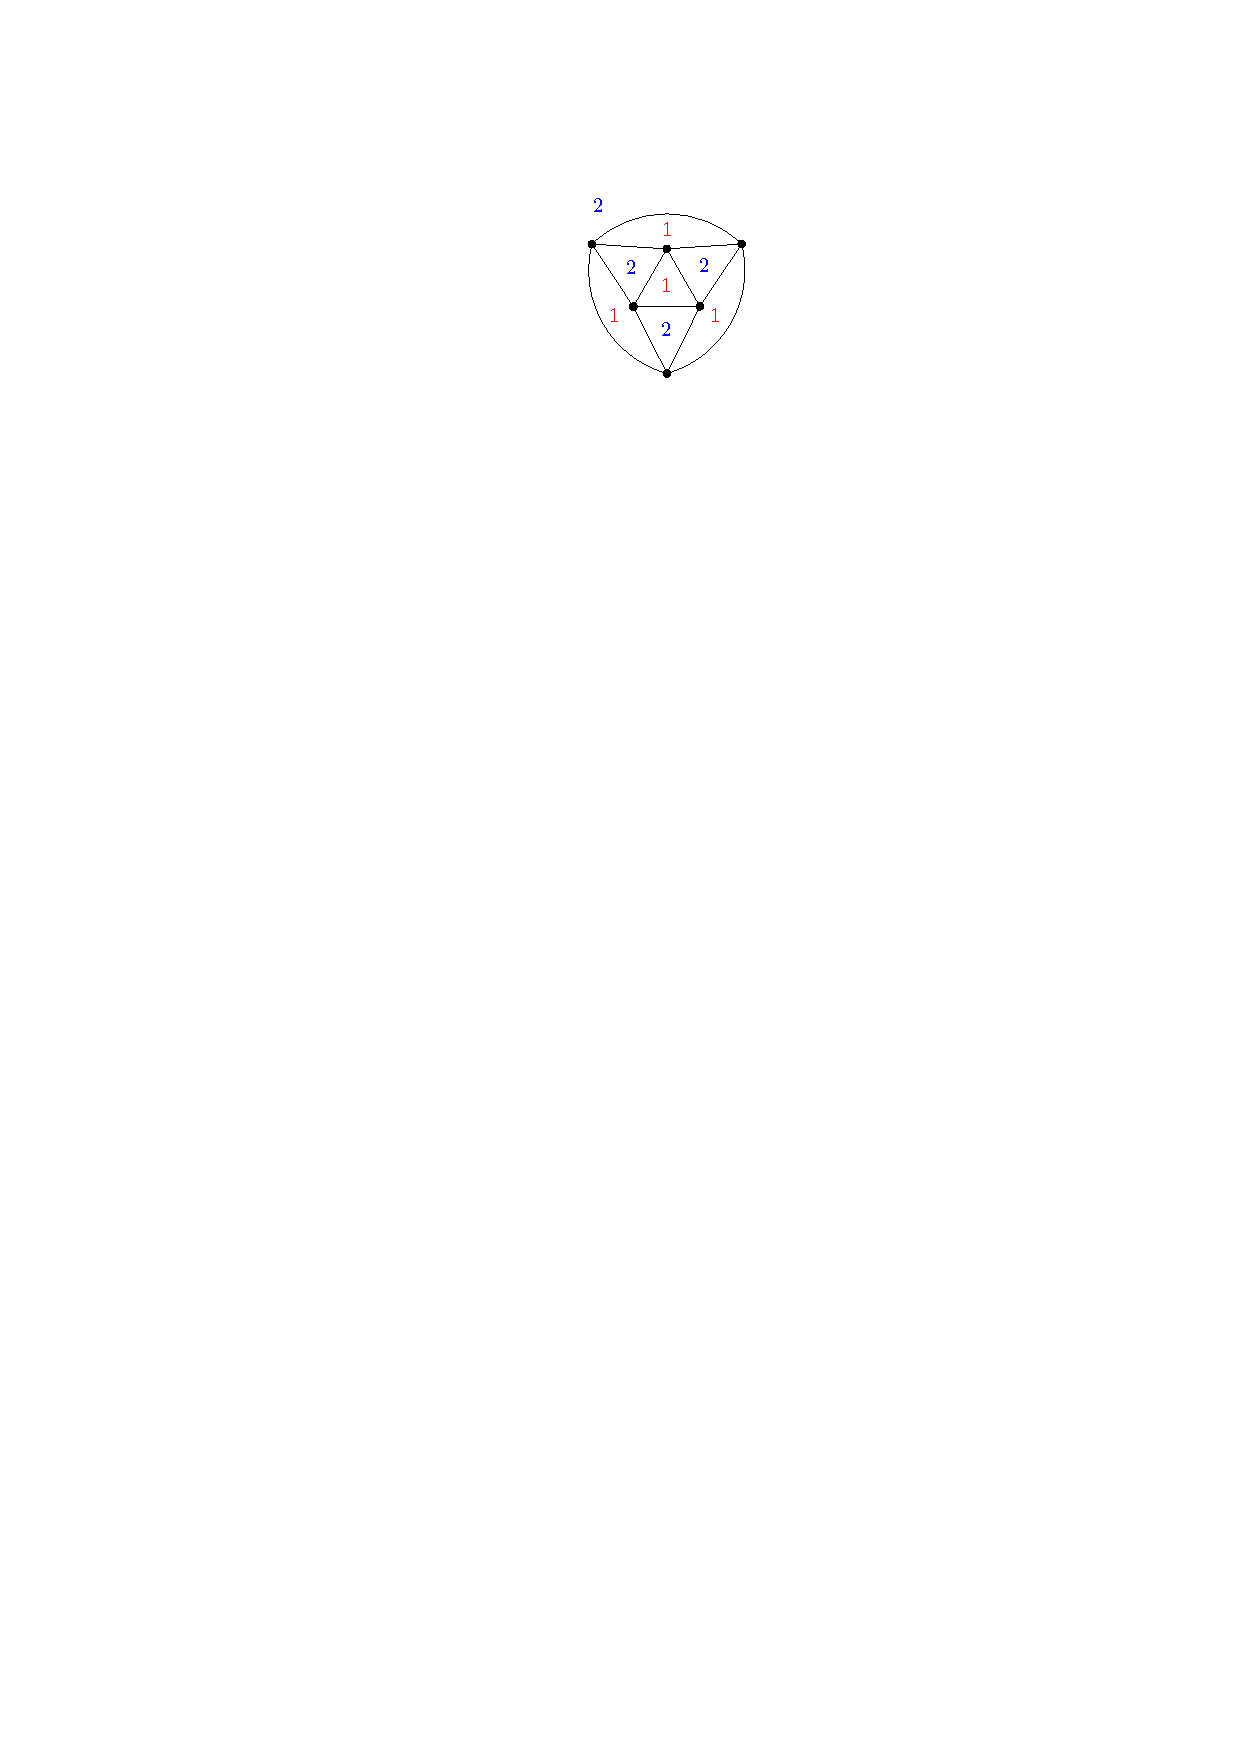
\includegraphics[width=0.2\textwidth]{../Resources/Figs/octahedral_face_colr.pdf}
    \caption{Face coloring of octahedral graph using two colors (1 and 2)}
    \label{fig:face_tot_coloring}
\end{figure}

\subsection{Rainbow coloring}

So far, the particular colorings we have considered were all quite similar to each other. In what sense? All of their coloring rules were based of the notion of adjacency of some elements i.e. neighboring vertices, incident edges etc. could not share the same color. There exists other types of colorings, where the coloring rules are based on other concepts such as connectivity. One such example is the \textit{rainbow coloring} \cite{chartrand08}.

\begin{definition}
    Let $S$ be a set. A \textit{rainbow coloring} of a plane graph $G=(V,E,F)$ is a coloring $c: E \rightarrow S$ belonging to family of colorings for which the coloring rule is: 
    \begin{equation}\label{eqn:rainbow_rule}
     \forall u,v \in V, \exists uv \text{-path } (u,e_1,w_1, \ldots ,w_{n-1},e_n,v) \text{ s.t. } \forall i \neq j : c(e_i) \neq c(e_j) \tag{$R_R$}
    \end{equation}
    We will denote this family of colorings by $X^R$.
\end{definition}

\begin{figure}[H]
    \centering
    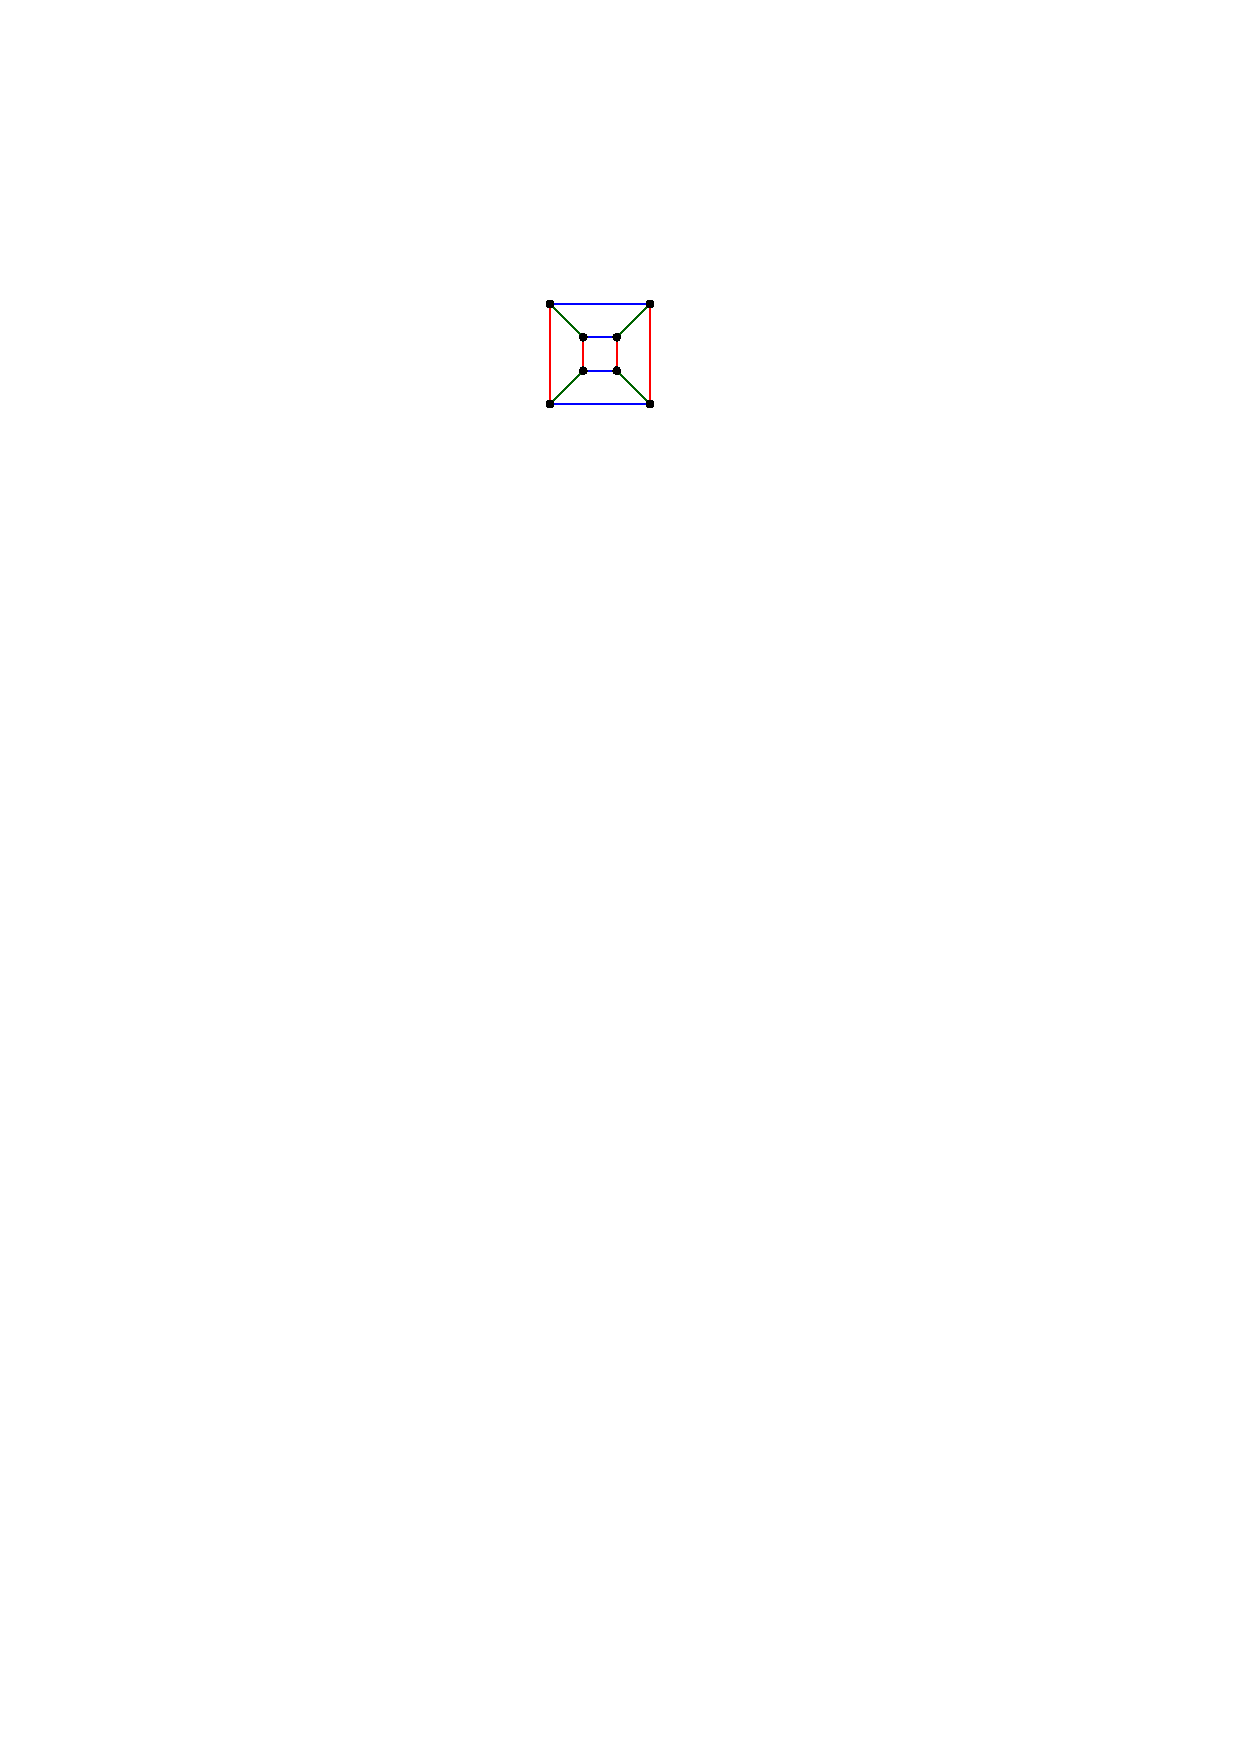
\includegraphics[width=0.2\textwidth]{../Resources/Figs/cubical_edg_colr.pdf}
    \caption{Rainbow coloring of cubical graph. Let us appreciate the fact, that it is also an edge coloring.}
    \label{fig:cubical_rainbow_coloring}
\end{figure}

\begin{figure}[H]
    \centering
    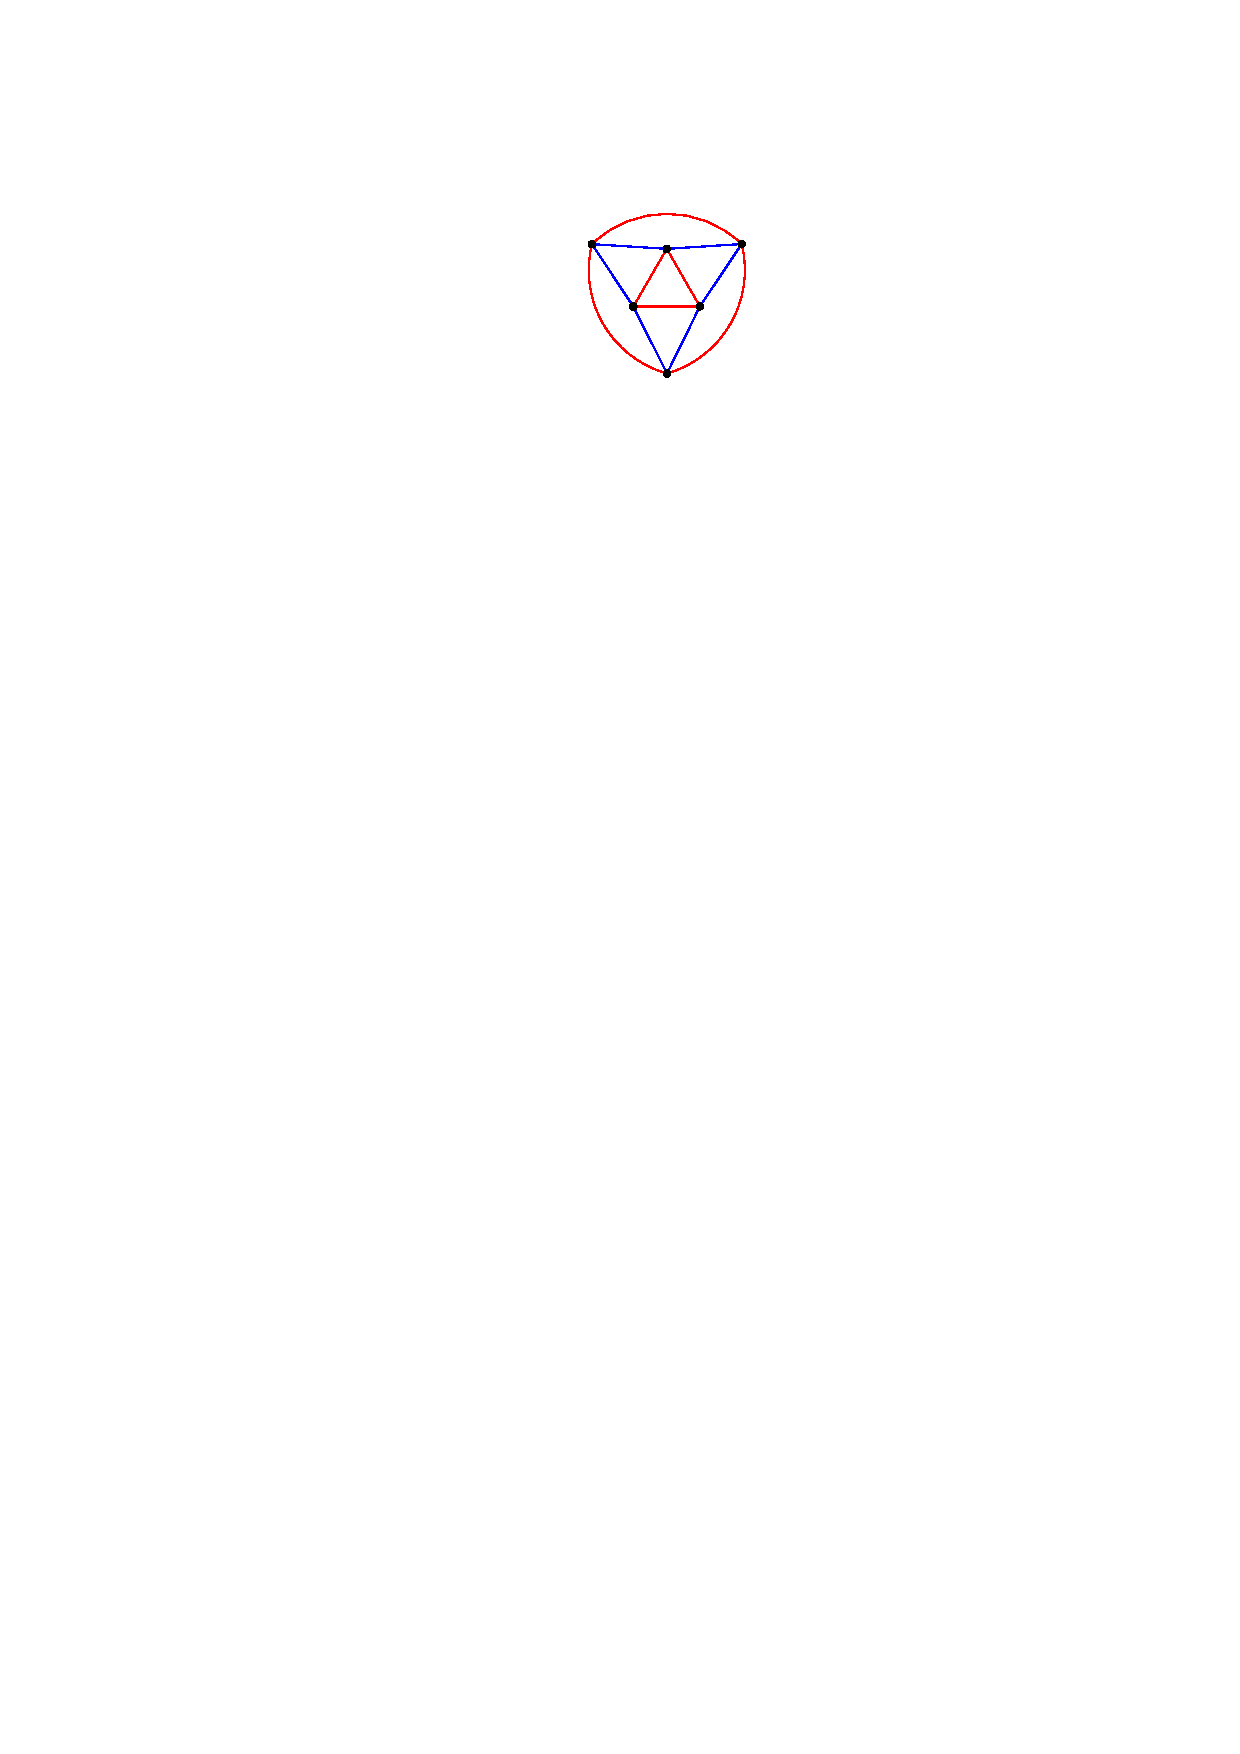
\includegraphics[width=0.2\textwidth]{../Resources/Figs/octahedral_rainbow_colr.pdf}
    \caption{Rainbow coloring of octahedral graph. Note, that it is not a valid edge coloring.}
    \label{fig:octahedral_rainbow_coloring}
\end{figure}

\subsection{Magic labeling}

There exists also coloring rules, that are based on the actual values of the colors. In that case, the colors cannot be any set of arbitrary elements, but must correspond to a subset of natural numbers, where we have a meaningful definition of addition operation on the colors. In that case, the colorings are usually referred to as \textit{labelings}.

\begin{highlight}

All of the labelings share a notion of assigning a \textit{weight} to the elements of a graph. For element $x$, we denote this weight by $w(g)$. Using this notation, we can define \textit{edge-labeling} more precisely as a function $l:E \rightarrow \mathbb{N}$ and analogously \textit{vertex-labeling} as a function $l:V \rightarrow \mathbb{N}$

Moreover we call an edge-labeling \textit{magic} if $\exists k \in \mathbb{N} : \forall v \in V:w(v) = k$ where $w$ is an arbitrary function in terms of $l$. In other words, the edge-labeling $l$ is magic if all the vertices have the same weight when the edges are labeled using $l$. For example, we might define $w(v) = \sum_{uv \in E}l(uv)$. Analogous definition holds for magic vertex-labeling.

All the definitions of labelings above are based on a book called \textit{Magic Graphs} by Wallis \cite{marrwall2013}.

\end{highlight}

\vspace{5pt}
\todo[inline]{IDEA: Add definition of perfect coloring}